
\newcommand{\FigOverview}{
\begin{figure}[t]
    \centering
    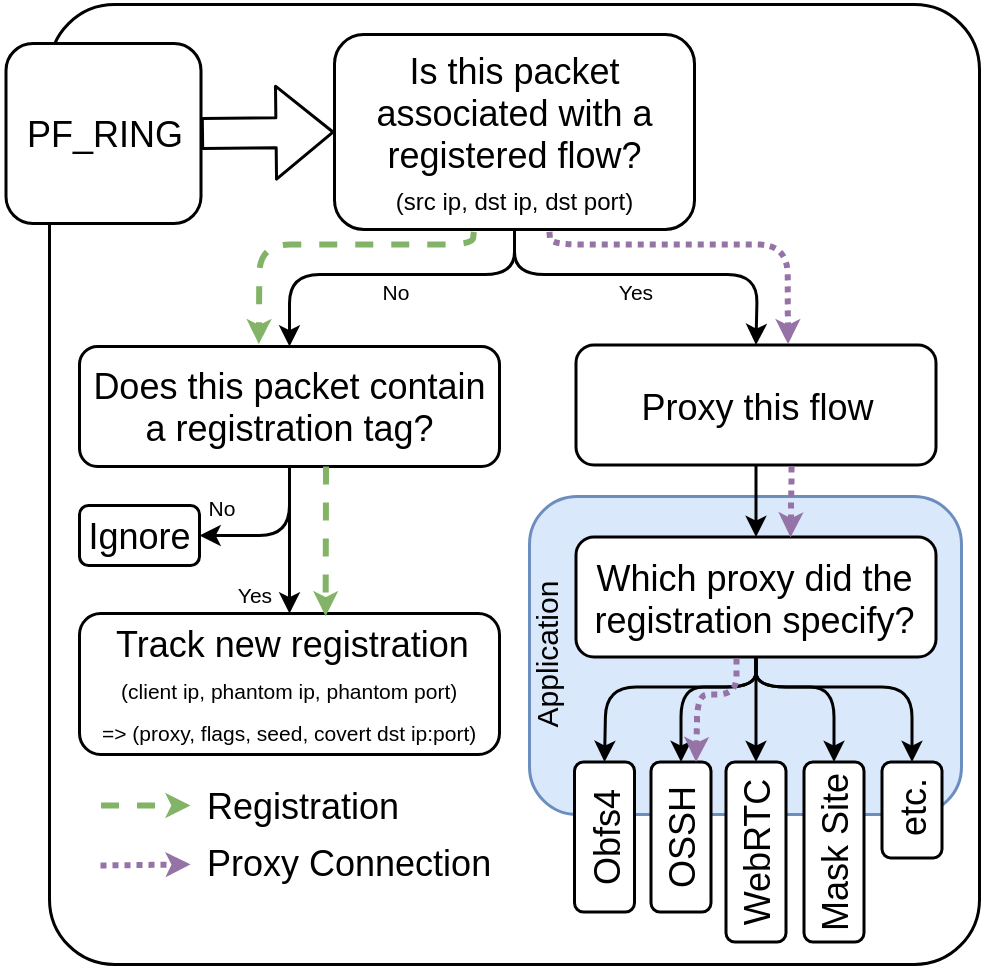
\includegraphics[width=\linewidth,clip]{figures/dark-decoy-flow2.png}
    \caption{\textbf{\scheme Operations}\,---\,\rm%
        A \scheme session is constructed in two pieces. First a client registers by sending a tls connection
        to the Decoy host (see Figure 2c) with a steganographically tagged payload.
        This registration contains the true address that the client would like to connect to and a seed 
        which the \scheme station uses to derive the Phantom IP address for the session(green dashed flow). 
        Second The client derives the same 
        Phantom IP address and connects directly to it using the proxy protocol (e.g. OSSH) that they specified in
        their registration (purple dotted flow). The station identifies registered packets by source IP, destination IP,
        and destination port (client IP, phantom IP, and phantom port respectively). The traffic is passed 
        to a proxy server handling the specific proxy specified by the client then redirected to the 
        covert address that the client indicated in their registration. 
        \\\hspace{\textwidth}
        Secrets for the individual proxy services are shared out of band or derived from the shared secret 
        between the client and the station such that an adversary attempting to probe a connection will be
        unable to connect to the proxy service. 
    }
    \label{fig:overview}
\end{figure}
}

\newcommand{\FigHighLevel}{
\begin{figure}[]
    \centering
    %\vspace{-0.54in}
    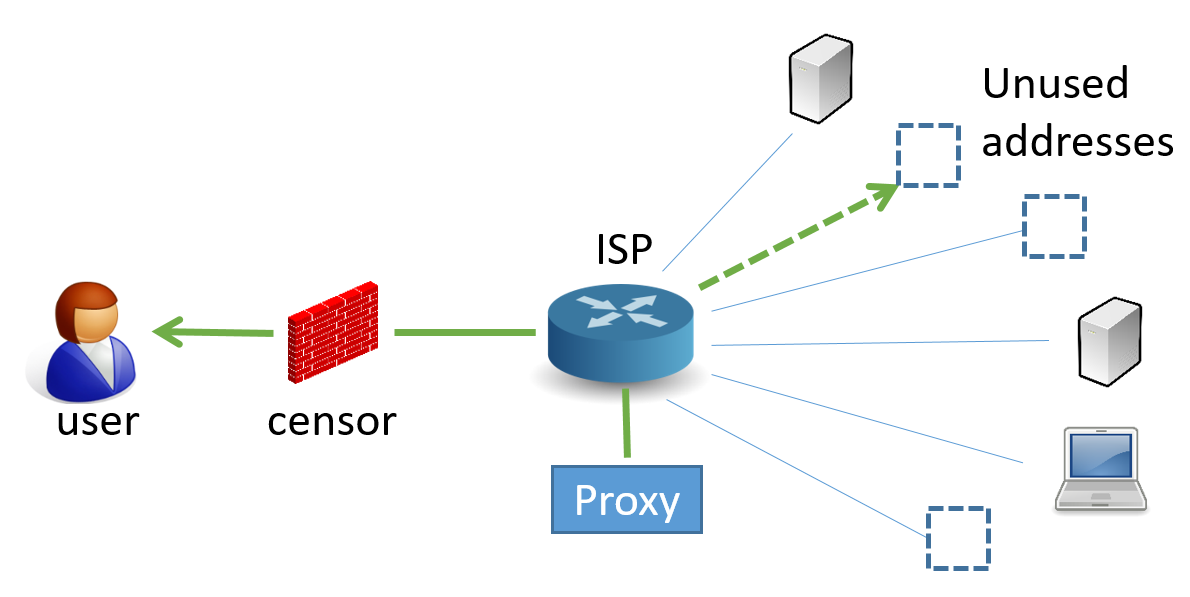
\includegraphics[width=\linewidth,clip]{figures/high-level.png}
    \caption{\textbf{\scheme Overview}\,---\,\rm%
      An ISP deploys a \scheme station, which sees a passive tap of passing traffic.
      Following a steganographic registration process, a client can connect
      to an unused IP address in the ISP's AS, and the station will
      inject packets to communicate with the client as if there were a proxy server at that address.
    }
    \label{fig:highlevel}
\end{figure}
}

\newcommand{\FigUpload}{
\begin{figure}[t]
    \centering
    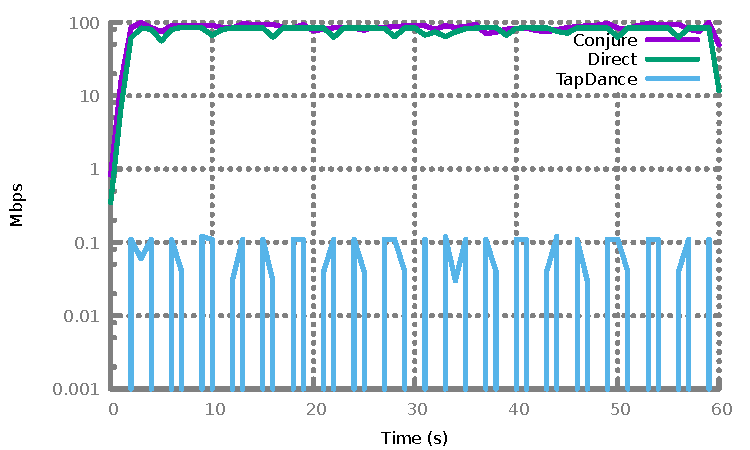
\includegraphics[width=0.95\linewidth,clip]{figures/bandwidth-up.pdf}
    \caption{\textbf{Upload Performance}\,---\,\rm%
        We used iperf to measure the upload bandwidth for a direct connection, TapDance, and \scheme.
        As expected, TapDance's upload performance is several orders of magnitude lower than
        the link capacity, due to the overhead of frequent reconnects to the decoy.
    }
    \label{fig:upload}
\end{figure}
}

\newcommand{\FigDownload}{
\begin{figure}[t]
    \centering
    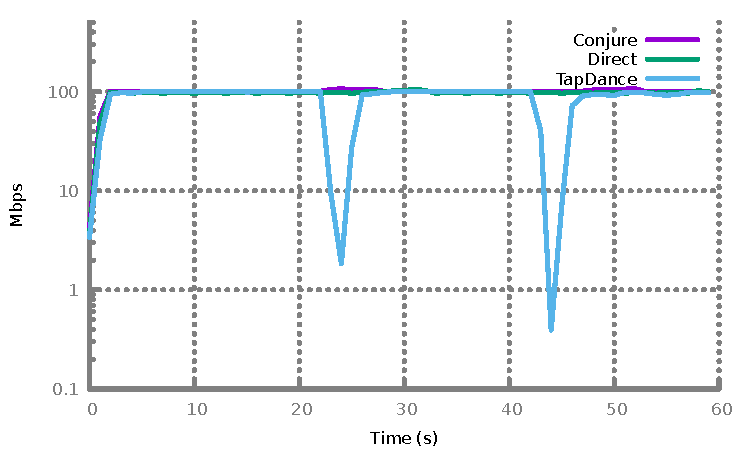
\includegraphics[width=0.95\linewidth,clip]{figures/bandwidth-down.pdf}
    \caption{\textbf{Download Performance}\,---\,\rm%
        Using iperf, we compare the download performance of a direct connection, TapDance, and \scheme.
        While TapDance can achieve link capacity download, it still has to occasionally reconnect
        to the decoy, as seen by the periodic dips. These reconnects are more common the more data
        the client sends (e.g. requests or any upload data).
    }
    \label{fig:download}
\end{figure}
}



\newcommand{\FigLatency}{
\begin{figure}[t]
    \centering
    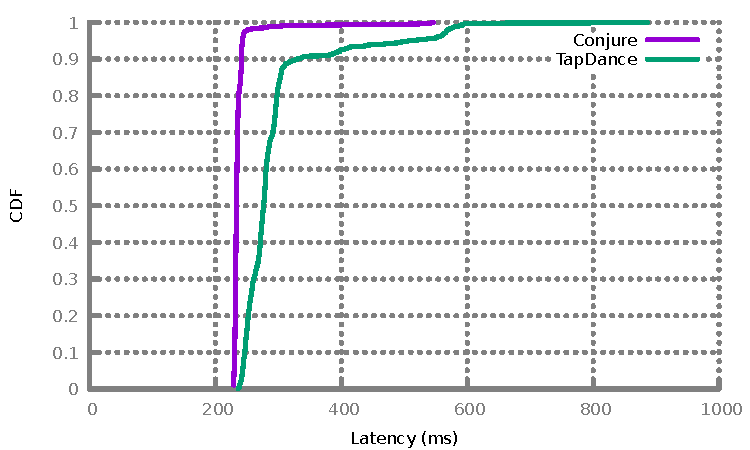
\includegraphics[width=0.95\linewidth,clip]{figures/td-dd-latency.pdf}
    \caption{\textbf{Latency}\,---\,\rm%
        We compare the CDF of latency for requests between \scheme and TapDance.
        In each case, we have a long-lived session over which requests are being made
        using Apache Benchmark (ab). At the median, \scheme has 44~ms (19\%) faster latency than
        TapDance.
        In addition, TapDance requests are frequently slowed by its intermittent reconnections
        to the decoy, as shown in the longer tail of TapDance's latency CDF. \scheme has no such
        reconnects, and thus has more uniform latency. At the 99th
        percentile, \scheme is 281~ms (92\%) faster than TapDance.
    }
    \label{fig:latency}
\end{figure}
}




\newcommand{\FigTapBandwidth}{
\begin{figure*}[ht]
    \centering
    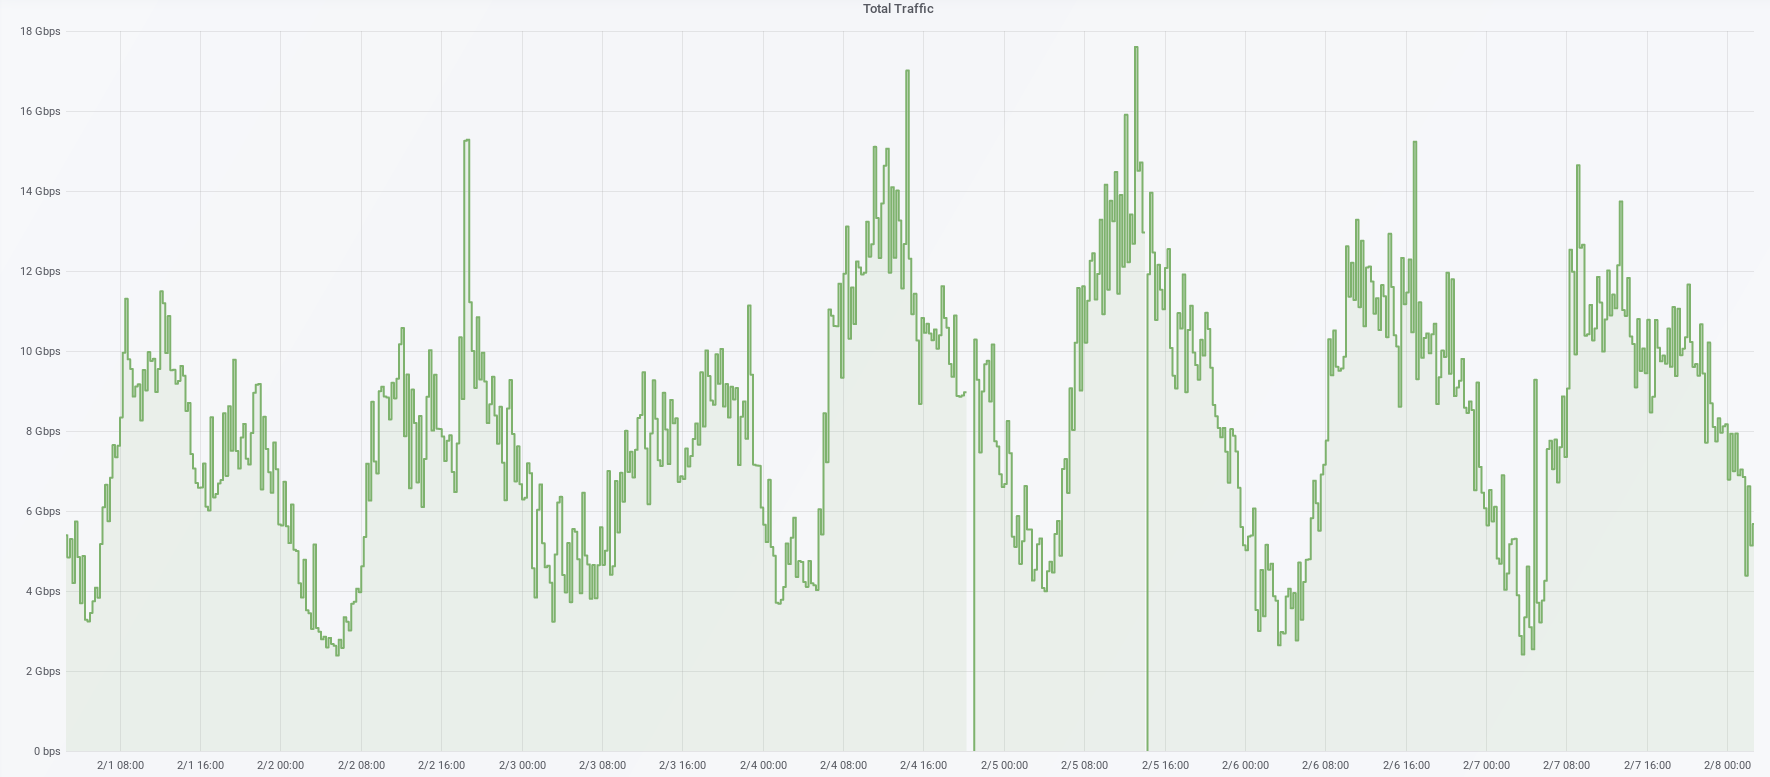
\includegraphics[width=0.75\linewidth,clip]{figures/decoy-tap-bandwidth.png}
    \caption{\textbf{Tap Bandwidth}\,---\,\rm%
        We deployed our \scheme implementation in a realistic ISP testbed on a
        tap of a 20~Gbps router. As shown in a typical week, traffic
        ranges from 2-17~Gbps.
    }
    \label{fig:tap-bandwidth}
\end{figure*}
}


\newcommand{\FigIpEntropy}{
\begin{figure}[t]
    \centering
    %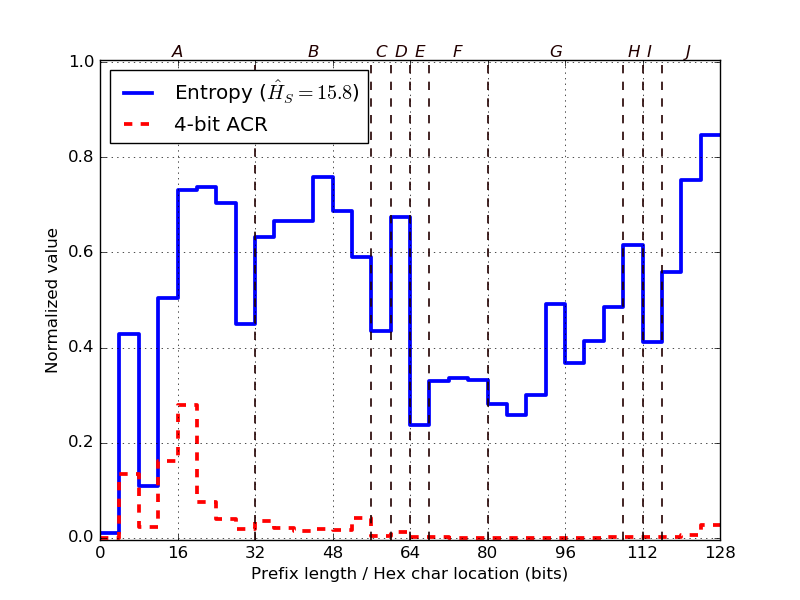
\includegraphics[width=\linewidth,clip]{figures/entropy_curveball_1hr.png}
    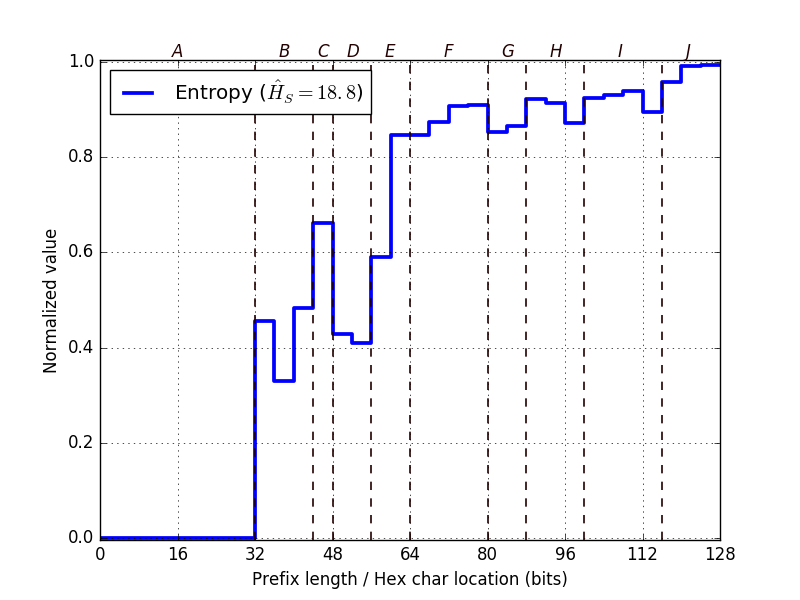
\includegraphics[width=\linewidth,clip]{figures/entropy-ip-16hr.png}
    \caption{\textbf{IPv6 Entropy}\,---\,\rm%
        Censors may be able to distinguish random-looking phantom host IPv6 addresses
        from legitimately used ones based on the address's entropy.
        We used the Entropy/IP tool~\cite{foremski2016entropy} to analyze the entropy
        of 4013 IPv6 addresses observed by our tap. This plot from the tool shows the
        normalized entropy of each nibble in the addresses, which is fairly high
        for most of the non-network prefix nibbles. In total, these addresses have
        about 75~bits of entropy (out of 96 expected), and the relatively high entropy
        present in each nibble would make it difficult for a censor to block without
        significant false positives / negatives. While distinguishable from random
        given enough samples,
        we can also use the Entropy/IP tool to generate addresses from the Bayesian Network
        model it produces.}
    \label{fig:ipentropy}
\end{figure}
}

\newcommand{\FigIpBits}{
\begin{figure}[t]
    \centering
    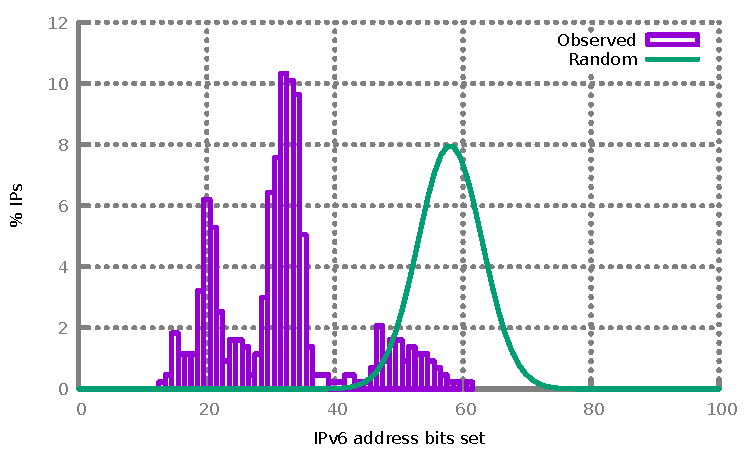
\includegraphics[width=\linewidth,clip]{figures/ip-bits-set-pdf.pdf}
    \caption{\textbf{IPv6 bits set}\,---\,\rm%
        We measure the number of bits set to 1 in IPv6 addresses in our ISP's /32
        and observed by our tap,
        and compare it to the Binomial distribution (Random) we would expect to see
        if the 96 non-network bits of each address were chosen randomly. In practice,
        we observe much fewer bits set.
        Nonetheless, the significant overlap of these distributions
        would make it difficult for censors to block any individual phantom hosts
        without collateral risk of blocking legitimate services.
       % suggesting that censors might be able to distinguish between phantom host addresses
        % and legitimate ones.
        %We note there are several /64 subnets that had many
        %addresses that appeared random (visibly overlapping the random distribution).
    }
    \label{fig:ipbits}
\end{figure}
}


\newcommand{\yes}{\CIRCLE}
\newcommand{\no}{\Circle}
\newcommand{\maybe}{\LEFTcircle}

\newcommand{\TabCompare}{
\begin{table*}[t]
    \centering
    \begin{tabular}{l|cccccccc}
            % Multiflow? Waterfall?
            & \rot{Telex~\cite{telex11}} &
            \rot{Cirripede~\cite{cirripede11}} &
            \rot{Decoy Routing~\cite{curveball11}} &
            \rot{TapDance~\cite{tapdance14}} & \rot{Rebound~\cite{rebound15}} & \rot{Slitheen~\cite{slitheen16}} & \rot{Waterfall~\cite{waterfall17}} & \rot{\textbf{\scheme}} \\
            \hline
                                      %Telex Cirr  DR     TD      RB    Slth   Water  DD
            No inline blocking        & \no & \no  & \no & \yes  & \no  & \no  & \no  & \yes \\
            Handles asym.\ routing     & \no & \yes & \no  & \yes & \yes & \no  & \yes & \yes \\
            %Currently deployed        & \no & \no  & \no  & \yes & \no  & \no  & \no  & \no \\
            Replay attack resistant   &\yes & \yes & \yes & \no  & \yes & \yes & \yes & \yes \\
            Traffic analysis resistant &\no  & \no  & \no  & \no  &\maybe& \yes &\maybe& \no \\
            %Uses unused addresses     & \no & \no  & \no  & \no  & \no  & \no  & \no  & \yes \\
            Unlimited Session Length  &\yes & \yes & \yes & \no  & \no  & \no  & \no  & \yes \\
            %ISP Deployment           &\no  & \no  & \no  & \yes & \no  & \no  & \no  & \yes \\
    \end{tabular}
    \medskip
    \caption{\textbf{Comparing Refraction Networking schemes}\,---\,\rm%
        ``No inline blocking'' corresponds to schemes that can operate as a passive tap on the side
        without needing an inline element in the ISP network.
        ``Handles asymmetric routes'' refers to schemes that work when only one direction (either client to decoy or decoy to server) is seen by the station.
        ``Replay attacks'' refers to censors who may replay/preplay previous messages or actively probe
        the protocol.
        ``Traffic analysis'' includes latency, inter-packet timing, and website fingerprinting.
        ``Unlimited Sessions'' shows schemes that do not need to repeatedly reconnect to download
        or upload arbitrarily large content.}
    \label{tab:compare}
\end{table*}
}


\newcommand{\TabApplications}{
\begin{table}[t]
    \centering
    \begin{tabular}{l|ccccc}
            & \rot{OSSH~\cite{ossh}} &
              \rot{\texttt{obfs4}~\cite{obfs4}} &
              \rot{Mask Sites} &
              \rot{TLS eSNI} & \rot{WebRTC} \\
            \hline
            Active probe resistant  & \yes  & \yes & \yes & \yes & \yes \\
            Randomized or Tunneling & R    & R    & T    &  T   & T \\
            Known passive attack    & \cite{Fifield2017a} & \cite{wang2015seeing} & - & - & - \\
            \scheme implementation  & \yes & \no  & \yes  & \no & \no \\
    \end{tabular}
    \medskip
    \caption{\textbf{\scheme Applications}\,---\,\rm%
    ``Active probe resistant`` protocols are designed to look innocuous even if scanned by a censor.
    ``Tunneling`` (T) protocols use another protocol (e.g. TLS) to blend in, while ``Randomized`` (R)
        ones attempt to have no discernable protocol fingerprint or headers.
        For existing protocols, we list any known attacks suggested in the literature that let censors
        passively detect them. We also list if we have implemented the application in our prototype.}
    \label{tab:applications}
\end{table}
}

\newcommand{\FigImplementation}{
\begin{figure}[t]
    \centering
    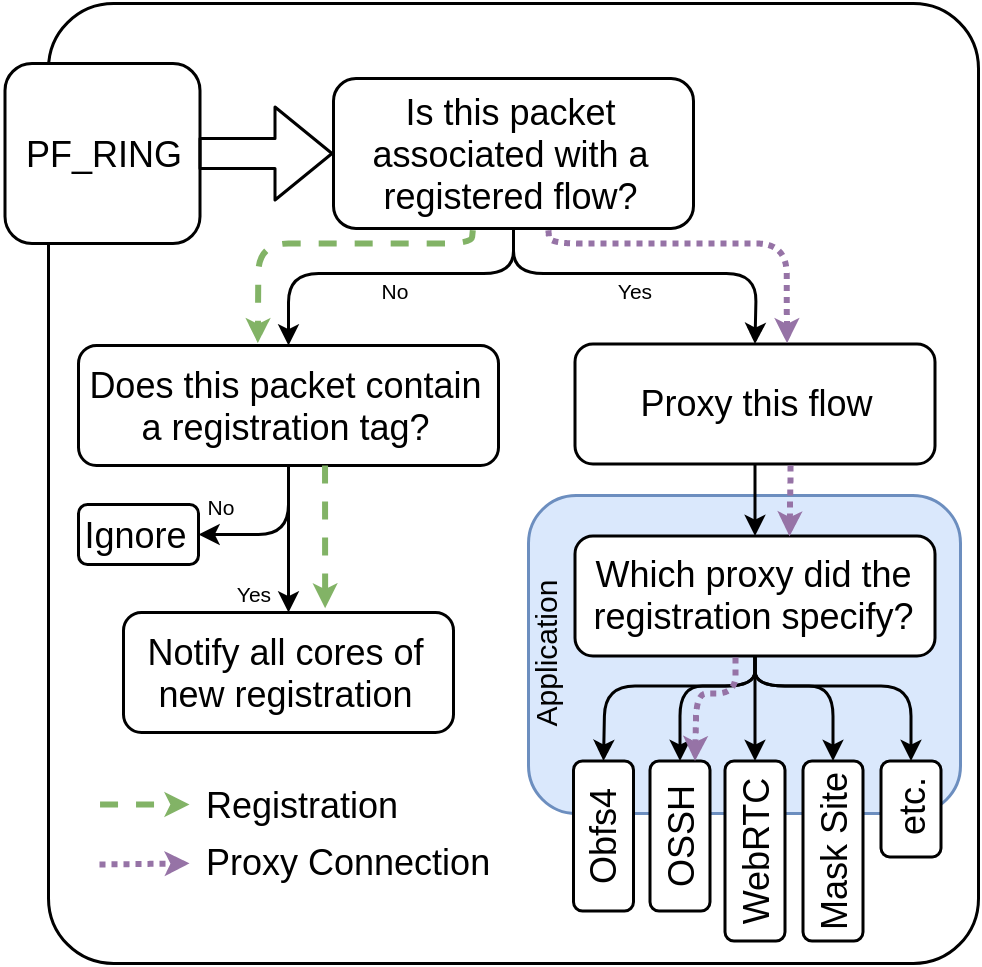
\includegraphics[width=0.7\linewidth,clip]{figures/dark-decoy-flow1.png}
    \caption{\textbf{Station Architecture}\,---\,\rm%
        We used PF\_RING to receive packets from a 20~Gbps packet tap, which we load balance
        across 4~CPU cores. The detector process identifies registrations, notifying all
        cores when a new registration is received (green dashed registration flow). The detector also
        identifies packets associated with registered flows (by connection 4-tuple) and diverts them
        to a local application which handles proxying connections(purple dotted flow). The local 
        application determines which proxy the flow should use based on a parameter specified by 
        the client in the registration and initializes a goroutine to handle forwarding. 
        \\\hspace{\textwidth}
        A censor trying to interfere in this
        connection would need to co-opt the clients IP address in a precise window (after the 
        registration but before the client connects to the phantom) and correctly guess the phantom hosts 
        IP address (or connect to all possible phantom IPs) before the active probe traffic gets to the local application. 
        At this point their connection will fail in a manor specific to the proxy that the client specified
        in the registration (e.g. connecting to OSSH without knowledge of the preshared secret).}
    \label{fig:implementation}
\end{figure}
}

\newcommand{\FigEvolution}{
\begin{figure}
  \centering
  \begin{subfigure}{\columnwidth}
    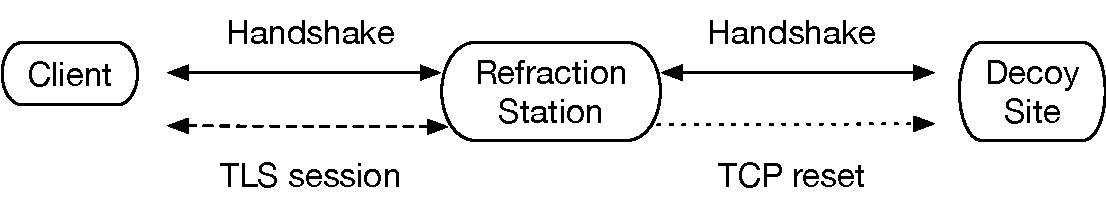
\includegraphics[width=\columnwidth]{figures/refraction-v1}
    \vspace{-3pt}

    \caption{\textbf{First generation systems}\rm for Refraction Networking, such as Telex and Cirripede, operated as inline network elements, with the ability to observe traffic and block specific flows. ISPs worried that if the inline element failed, it could bring down the network.\looseness=-1}
    \label{fig:refraction-v1}
  \end{subfigure}
  \vspace{16pt}

  \begin{subfigure}{\columnwidth}
    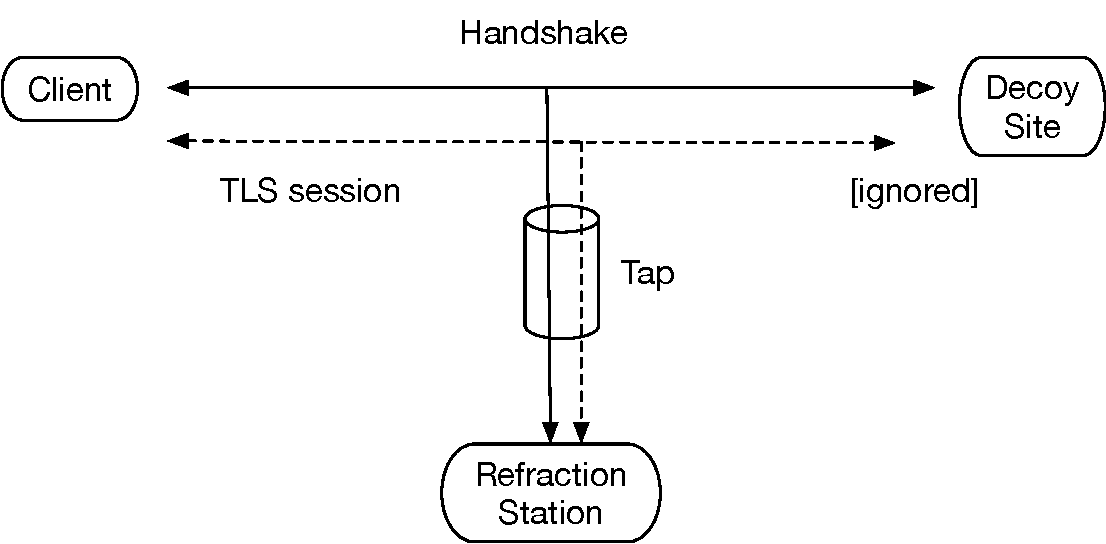
\includegraphics[width=\columnwidth]{figures/tapdance}
    \vspace{-3pt}

    \caption{\textbf{TapDance}\rm is a second-generation Refraction Network scheme that operates without flow blocking, needing only to passively observe traffic and inject packets. TapDance has recently been deployed at a mid-size ISP, but the techniques used to silence the decoy site and participate in the client--decoy TCP connection mid-stream add significant complexity, performance bottlenecks, and detection risk.}
    \label{fig:tapdance}
  \end{subfigure}
  \vspace{16pt}

  \begin{subfigure}{\columnwidth}
    \label{fig:evolutionconjure}
    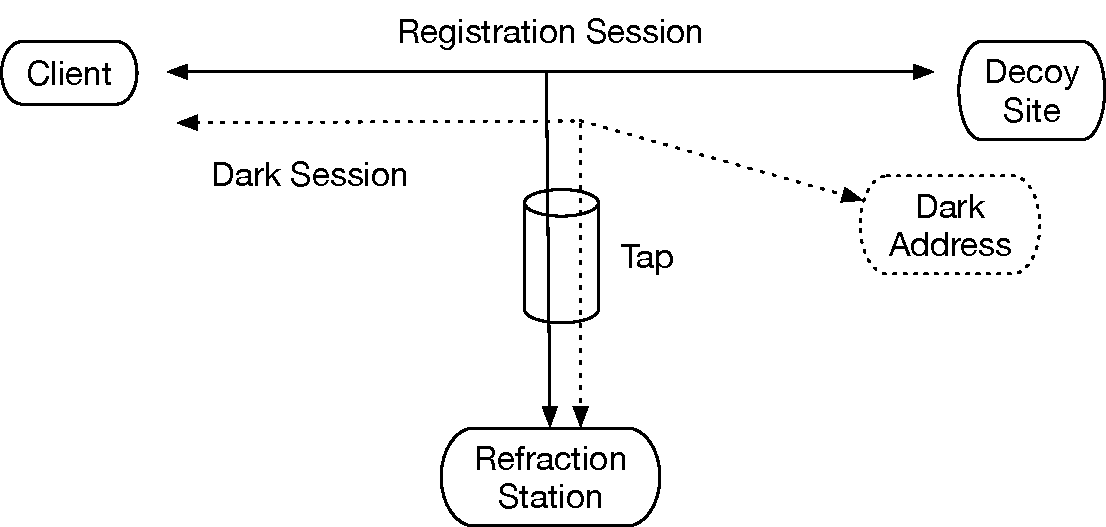
\includegraphics[width=\columnwidth]{figures/dark-decoys}
    \vspace{-3pt}

    \caption{\textbf{\scheme}\rm, our third-generation Refraction Networking design, overcomes these limitations.  It uses two sessions. First, the client connects to a decoy site and embeds a steganographic registration message, which the station receives using only a passive tap.  Second, the client connects to a ``phantom host'' where there is no running server, and the station proxies the connection in its entirety.}
    \label{fig:dark-decoys}
  \end{subfigure}

  \vspace{12pt}
  \caption{\textbf{Evolution of Refraction Networking}}
\end{figure}
}
